\chapter{Installation}
\label{chapter:Installation}
\index{Installation}

This section describes the process for installing OTB on your system. OTB is a toolbox, and as such, once it is installed in your computer, it provides by default a set of useful libraries. You can use these libraries to build your own applications based on it. What OTB does provide, besides the toolbox, is a large set of test files and examples that will introduce you to OTB concepts and will show you how to use OTB in your own projects.

Since the release 3.12, OTB embeds a specific framework to generate applications in a more user-friendly way. OTB provides for each application one shared library (also known as plugin). This plugin can be auto-loaded into appropriate tools without recompiling, and is able to fully describe its own parameters, behavior and documentation.

The tools to use these plugins can be extended, but OTB is shipped with the
following:
\begin{itemize}
\item A command-line launcher,
\item A graphical launcher, with an auto-generated Qt interface,
  providing ergonomic parameters setting, display of documentation,
  and progress reporting,
\item A C and SWIG interface, which means that any application can be
  loaded, set up and executed into a high-level language such as \textbf{Python}
  for instance.
\end{itemize}

Based on a visualization framework which used FLTK libraries, Orfeo ToolBox team provides an integrated application which giving graphical access to a lot of OTB functionalities: \textbf{Monteverdi}. Since mid-2013, we also provide a new graphical application based on Qt: \textbf{Monteverdi2}. This new application used the OTB-Applications tools as processing framework. 
   
There are two ways to install OTB library on your system: installing from a binary distribution or compiling from sources. The choice depends on your system, and on what you intend to do.


\section{Installing binary packages}
\label{sec:install_binaries}

You can find all information about the installation of binary packages for OTB-Applications, Monteverdi and Monteverdi2 (if they are available on your platform) into the OTB-Cookbook.

The binary packages for OTB library are only available on:
\begin{itemize}
\item Ubuntu 12.04 and higher
\item OpenSuse 12.X and higher
\item MacOSX through MacPorts software  
\end{itemize}

Currently, no OSGeo4W package is available for the OTB library, you need to build from source to use it on windows platform. However you can fund binary packages for Monteverdi, Monteverdi2 and OTB-Applications (command-line, QT based and python ones).


\section{Building from sources}
\label{sec:source}
OTB has been developed and tested across different combinations of operating systems, compilers, and hardware platforms including MS-Windows, Linux on Intel-compatible hardware and Mac OSX.  It is known to work with the following compilers in 32/64 bit:
\begin{itemize}
\item Visual Studio 2010 and higher compiler on MS-Windows
\item GCC 4.1 and higher on Unix/Linux systems
\item GCC on MacOSX (10.8 and higher) systems
\end{itemize}

Given the advanced usage of C++ features in the toolbox, some compilers may have difficulties processing the code. If you are currently using an outdated compiler this may be an excellent excuse for upgrading this old piece of software!

Please note that even if this section only describes how to compile OTB library and applications from sources, Monteverdi1 and Monteverdi2 can be compiled in a similar way.

In order to compile and install OTB, you need on your system:
\begin{itemize}
  \item \href{http://www.cmake.org/}{CMake} software (binary packages are available for most platforms).
  \item a compilers of the previous list.
 \end{itemize}

\subsection{Which libraries/packages are needed before compiling and installing OTB?}
The following table gathered the libraries (mandatory or not) used in the OTB. Some of them are included in the OTB but can be used as external libraries (this the default behavior if they are detected on your platform). 

\begin{center}
\begin{tiny}
\begin{table}[!htbp]
\begin{tabular}{|p{0.15\textwidth}|p{0.45\textwidth}|p{0.1\textwidth}|p{0.15\textwidth}|p{0.1\textwidth}|}
\hline
\textbf{Library} & \textbf{Web site} & \textbf{Mandatory} & \textbf{Where} & \textbf{Minimum version} \\
\hline
\textbf{ITK} & \url{http://www.itk.org} & yes & Intern/\textbf{Extern} & 4.5.0 \\
\hline
\textbf{GDAL} & \url{http://www.gdal.org} & yes & Extern & 1.10 \\
\hline
\textbf{OSSIM} & \url{http://www.ossim.org} & yes & \textbf{Intern}/Extern & 1.8.6 \\
\hline
\textbf{Curl} & \url{http://www.curl.haxx.se} & no & Extern & - \\
\hline
\textbf{FFTW} & \url{http://www.fftw.org} & no & Extern & - \\
\hline
\textbf{expat} & \url{http://expat.sourceforge.net/} & yes & Intern/\textbf{Extern} & - \\
\hline
\textbf{libtiff} & \url{http://www.libtiff.org} & yes & Extern & - \\
\hline
\textbf{libgeotiff} & \url{http://trac.osgeo.org/geotiff/} & yes & Extern & - \\
\hline
\textbf{OpenJPEG} & \url{http://code.google.com/p/openjpeg/} & no & Intern & - \\
\hline
\textbf{boost} & \url{http://www.boost.org} & no & Intern/\textbf{Extern} & - \\
\hline
\textbf{openthreads} & \url{http://www.openscenegraph.org} & no & Intern/\textbf{Extern} & - \\
\hline
\textbf{Mapnik} & \url{http://www.mapnik.org} & no & Extern & - \\
\hline
\textbf{tinyXML} & \url{http://www.grinninglizard.com/tinyxml} & yes & Intern/\textbf{Extern} & - \\
\hline
\textbf{KML} & \url{http://libkml.googlecode.com} & yes & Intern/\textbf{Extern} & - \\
\hline
\textbf{6S} & \url{http://6s.ltdri.org} & yes & Intern & - \\
\hline
\textbf{edison} & \url{http://www.caip.rutgers.edu/riul/} & yes & Intern & - \\
\hline
\textbf{SiftFast} & \url{http://libsift.sourceforge.net} & yes & Intern & - \\
\hline
\textbf{MuParser} & \url{http://www.muparser.sourceforge.net} & yes & Intern/\textbf{Extern} & - \\
\hline
\textbf{libSVM} & \url{http://www.csie.ntu.edu.tw/~cjlin/libsvm} & yes & Intern & - \\
\hline
\textbf{Qt} & \url{http://qt-project.org/} & no & Extern & 4 \\
\hline
\end{tabular}
\caption{Libraries used in the OTB. In the column Where, the default behavior during the configuration of OTB is indicated by when the status is bold. For example, by default external ITK library is used.}
\label{tab:installation2}
\end{table}
\end{tiny}
\end{center}

For windows user, some of these libraries can be found into the OSGeo4W installer.  

For Monteverdi, in addition to OTB, FLTK is required (\url{http://www.fltk.org}) as an external dependency. Therefore, you need to install it from your package manager or build it from source. For windows users, you can find it through the OSGeo4W installer.

For Monteverdi2, in addition to OTB, Qt4 (\url{http://qt-project.org/}) and Qwt5 (\url{http://qwt.sourceforge.net/}) are required as external dependencies. Therefore, you need to install them from your package manager or build them from source. For windows users, you can find them through the OSGeo4W installer.

You can find all the information to get and install these libraries directly from their respective website.

If you install external libraries through binary packages provided by your operating system or use system libraries, \textbf{be sure to also install libraries headers, which are mandatory to build OTB}.

\subsection{Getting a qualified Gdal library on Linux systems}\label{sec:gdal}

Gdal is a very rich data abstraction library, and there are many compilation time options in Gdal that will impact Gdal and therefore OTB libraries capabilities. There are also options and dependencies that could limit or prevent Orfeo ToolBox from working properly. On linux systems, there are a lot of Gdal binary packages with different configurations. It is therefore very important to know exactly your Gdal configuration before proceeding to the next step.

Here are the things to check:
\begin{itemize}
\item Gdal version (should be greater or equal to 1.10),
\item Gdal library should not expose any Tiff or Geotiff symbol (otherwise it may cause crashes in Orfeo ToolBox),
\item Gdal should support BigTiff (read or write Tiff files of more than 4 Gb).
\end{itemize}

\subsubsection{How to check if your Gdal qualifies for Orfeo ToolBox?}

If you already have a Gdal in your system (either from the official package manager of your distributions or from your own build), here is how to check if it qualifies for Orfeo ToolBox.

Gdal version can be checked using the following command:
\begin{verbatim}
$ gdal-config --version
\end{verbatim}

If version is lower than 1.10.0, you should build or install an up-to-date Gdal library.

If you have several versions of Gdal installed in your system, be sure to run this command for the version you intend to. You can check this with:
\begin{verbatim}
$ which gdal-config
\end{verbatim}

Next step is to check if the Gdal library leaks any Tiff or Geotiff symbol. First you need to locate gdal library. If it has been installed system wide, the library will most probably be located in \texttt{/usr/lib}. Otherwise, you need to find where is \texttt{libgdal.so}.

Once you found it, run:
\begin{verbatim}
$ nm -D libgdal.so | grep XTIFFOpen
\end{verbatim}

This should show either nothing, or the following:

\begin{verbatim}
00000000004b1100 T gdal_XTIFFOpen
\end{verbatim}

If the command outputs the following:

\begin{verbatim}
00000000004b1100 T XTIFFOpen
\end{verbatim}

It means that your Gdal library leaks Tiff and Geotiff symbols. Depending on your system, this might cause random crashes in Orfeo ToolBox when reading or writing Tiff images. In this case it is advised to build or retrieve a Gdal library that does not exhibit this issue.

Last, it might be important for you to be able to read and write Tiff files of more than 4 Gb with Orfeo ToolBox. To check for BigTiff file support, choose an image on your computer and run:
\begin{verbatim}
$ gdal_translate -co "BIGTIFF=YES" my_image.png my_image.tif
\end{verbatim}

If this fails, your Gdal library or the Tiff library it is linked to does not support BigTiff files. In this case it is advised to build or retrieve a Gdal library.

\subsection{Distributions and binary packages repositories known to distribute a qualified Gdal}

Among the different distributions and packages repositories that distribute a qualified Gdal, one can cite:
\begin{itemize}
\item The ubuntu-gis unstable ppa (\href{https://launchpad.net/~ubuntugis/+archive/ubuntugis-unstable}),
\item Default package for Ubuntu greater or equal to 14.04.
\end{itemize}

\subsection{Building your own qualified Gdal}

If do not yet have a Gdal library or suspect that the library you have will not qualify, you can build your own library. After downloading the latest version of gdal source code, run:

\begin{verbatim}
$ export GDAL_INSTALL_DIR=$HOME/local
$ ./configure --prefix=$GDAL_INSTALL_DIR \
  --with-geotiff=internal  \
  --with-rename-internal-libtiff-symbols=yes \
  --with-rename-internal-libgeotiff-symbols=yes
$ make install
\end{verbatim}

The \texttt{GDAL\_INSTALL\_DIR} environment variable allows to choose where you will install your Gdal library. It is NOT advised to install it system wide. It is recommended to choose a dedicated directory in your home folder. The configuration options will ensure that Gdal will build internal Tiff and Geotiff libraries that supports BigTiff files, while renaming their symbols so that they will not be leaked outside of the library. Depending on your need, feel free to enable more Gdal configuration options.

Once this is done, be sure to update your environment variables:
\begin{verbatim}
$ export PATH=$PATH:$GDAL_INSTALL_DIR/bin
$ export LD_LIBRARY_PATH=$LD_LIBRARY_PATH:$GDAL_INSTALL_DIR/lib
$ export GDAL_DATA=$GDAL_INSTALL_DIR/share/gdal
\end{verbatim}

Also note that with this Gdal configuration, you will still need to have Tiff and Geotiff libraries and headers available on your system to build OTB (due to third parties requiring them). However, you can use the system packages for those.

\subsection{Getting the OTB source code}

There are three ways of getting the OTB source code:
\begin{itemize}
\item Download the latest current release from the \href{http://sourceforge.net/projects/orfeo-toolbox/}{OTB download page},
\item Clone the current release with \href{http://mercurial.selenic.com}{Mercurial} from the \href{http://hg.orfeo-toolbox.org/OTB}{OTB mercurial server},
\item Clone the latest revision with \href{http://mercurial.selenic.com}{Mercurial} from the \href{http://hg.orfeo-toolbox.org/OTB}{OTB mercurial server}.
\end{itemize}

These last two options need a proper \href{http://mercurial.selenic.com}{Mercurial} installation. To get source code from Mercurial, do:
\begin{verbatim}
hg clone http://hg.orfeo-toolbox.org/OTB
\end{verbatim}

Using Mercurial, you can easily navigate through the different version. For instance, this brings you to the 3.16.0 source code version:
\begin{verbatim}
hg update -r 3.16.0
\end{verbatim}

And this brings you to the latest development version:
\begin{verbatim}
hg update
\end{verbatim}


\subsection{Configuring OTB}
\label{sec:ConfiguringOTB}

\index{Configuration}

The challenge of supporting OTB across platforms has been solved through the use of CMake, a cross-platform, open-source build system. CMake is used to control the software compilation process using simple platform and compiler independent configuration files.  CMake generates native makefiles and workspaces that can be used in the compiler environment of your choice. CMake is quite sophisticated: it supports complex environments requiring system configuration, compiler feature testing, and code generation.

CMake generates Makefiles under UNIX systems and generates Visual Studio workspaces under Windows (and appropriate build files for other compilers like Borland). The information used by CMake is provided by \code{CMakeLists.txt} files that are present in every directory of the OTB source tree. These files contain information that the user provides to CMake at configuration time. Typical information includes paths to utilities in the system and the selection of software options specified by the user.

\subsubsection{Preparing CMake}
\label{sec:CMakeforOTB}

\index{CMake}
\index{CMake!downloading}

CMake can be downloaded at no cost from
\begin{center}
  \url{http://www.cmake.org}
\end{center}

OTB requires at least CMake version 2.8.6. You can download binary versions for most of the popular platforms including Windows, Solaris, IRIX, HP, Mac and Linux. Alternatively you can download the source code and build CMake on your system. Follow the instructions in the CMake Web page for downloading and installing the software.

\index{CMake!OTB tree}
Running CMake initially requires that you provide two pieces of
information:
\begin{itemize}
\item Where the source code directory is located (ex.: OTB\_SOURCE\_DIR),
\item Where the object code is to be produced: (ex.: OTB\_BINARY\_DIR).
\end{itemize}
These are referred to as the \emph{source directory} and the \emph{binary directory}.
We recommend setting the binary directory to be different than the source directory (an
\emph{out-of-source} build), but OTB will still build if they are set
to a directory inside the source directory (an \emph{in-source} build).

\subsubsection{Compiling OTB}
CMake runs in an interactive mode in that you iteratively select
options and configure according to these options. The iteration
proceeds until no more options remain to be selected. At this point, a
generation step produces the appropriate build files for your
configuration.

This interactive configuration process can be better understood if you
imagine that you are walking through a decision tree.  Every option that you
select introduces the possibility that new, dependent options may become
relevant. These new options are presented by CMake at the top of the options
list in its interface.  Only when no new options appear after a configuration
iteration can you be sure that the necessary decisions have all been made. At
this point build files are generated for the current configuration.

As the following figures display it, CMake has a different interface according to your systems.
\label{sec:ConfiguringOTBwithVTK}
\index{Configuration!with VTK}

\begin{figure}[ht]
\centering
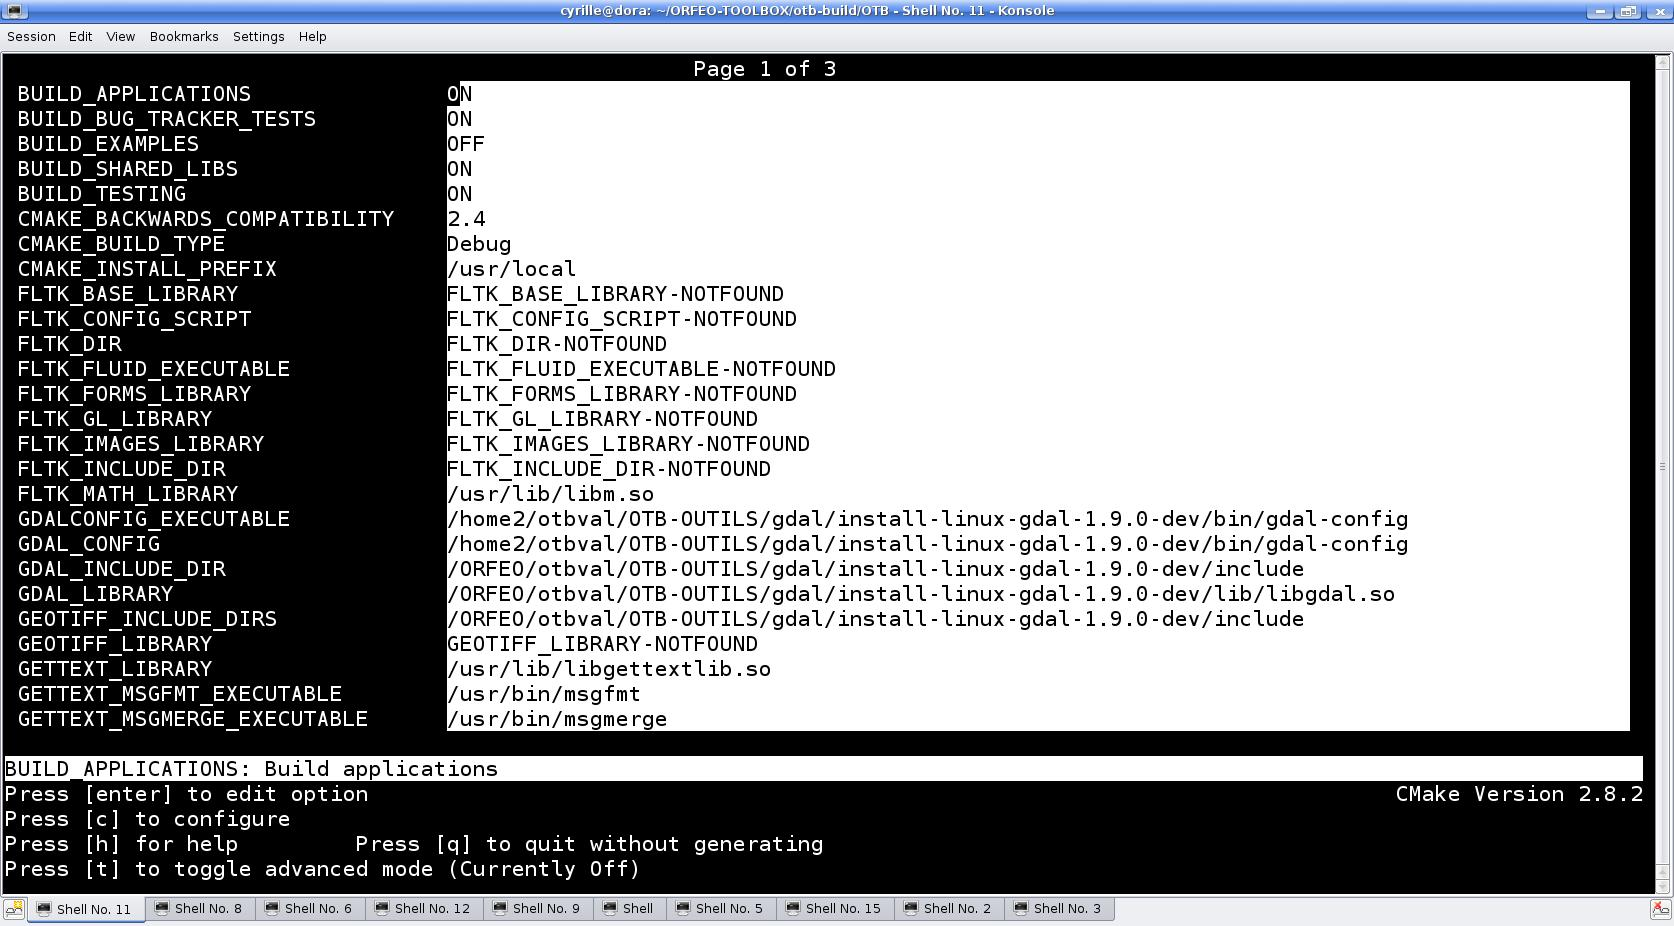
\includegraphics[width=0.8\textwidth]{ccmakeScreenShot.eps}
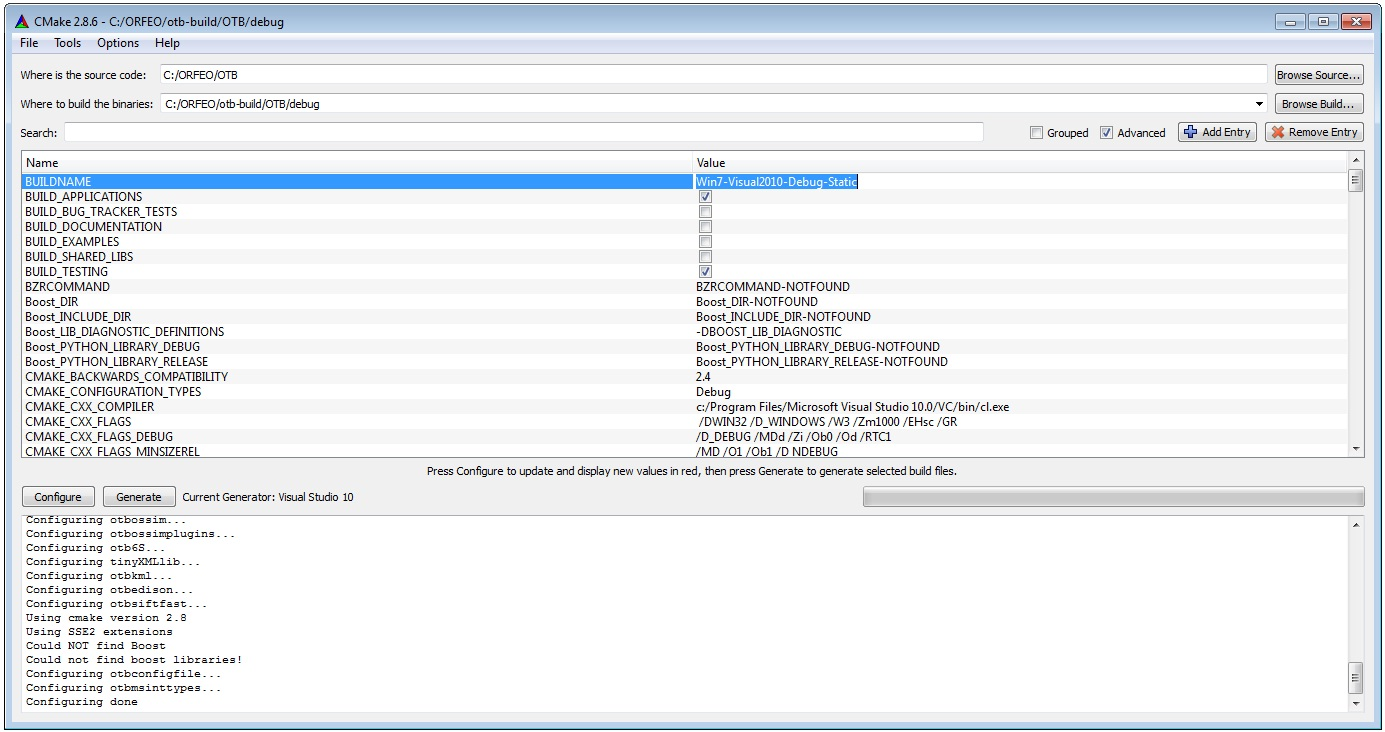
\includegraphics[width=0.8\textwidth]{CMakeSetupScreenShot.eps}
\itkcaption[Cmake user interface]{CMake interface. Top) \texttt{ccmake}, the UNIX
version based on \texttt{curses}. Bottom) \texttt{CMakeSetup}, the MS-Windows
version based on MFC.}
\label{fig:CMakeGUI}
\end{figure}


\textbf{\underline{On Windows:}}
\index{Preliminary steps}

The OTB needs some external libraries to work, as described in the table \ref{tab:installation2}. To manage correctly and easily the dependencies of OTB under Windows we strongly recommend to install \href{http://trac.osgeo.org/osgeo4w/}{OSGeo4W} tool. This software will provide you with all the necessary dependencies in 32 bit and 64 bit mode. Please follow these steps:
\begin{enumerate}
\item  Download the installer setup (32/64bit)
\item  Run the setup installer with Admin Rights
\item  Select Advanced Install
\item  Select Install from Internet
\item  Keep as much as possible the default values about root directory and other parameters. You must have the write access to this root directory. 
\item  In the next screen, select a local package directory (idem you must have the write access to this directory)
\item  Select your Internet connection settings
\item  Select the default download site
\item  Select the following packages:
	\begin{itemize}
	\item  msvcrt
	\item  gdal
	\item  curl
	\item  expat 
	\item  ossim
	\item  opencv
	\item  qt4-devel
	\item  swig
	\item  python
	\item  fftw-devel
	\item  libtiff
	\end{itemize}
\item  Run the installation process
\item  Accept all the dependencies required by the selected packages
\item  Wait the downloading and the installation of the packages
\end{enumerate}

Create a directory, where you have write access, to store your work (for example at C:\textbackslash path\textbackslash to\textbackslash MyOTBDir).
Organize your directories as it :
\begin{itemize}
\item MyOTBDir\textbackslash src
\item MyOTBDir\textbackslash build
\item MyOTBDir\textbackslash install
\end{itemize}

Retrieve the latest release of OTB (you can find the latest source \href{http://sourceforge.net/projects/orfeo-toolbox/files}{here}) and unzip it into the previous source directory.


\index{Configure, Build and Install OTB}

We will describe here how to compile and install the library with the main functionalities in Release and ReleaseWithDebugInfo mode.
Create an OTB.bat file into your MyOTBDir and copy paste the following lines:

\begin{verbatim}
@echo off

call "C:\Program Files (x86)\Microsoft Visual Studio 10.0\Common7\Tools\vsvars32.bat"

set /A ARGS_COUNT=0    
for %%A in (%*) do set /A ARGS_COUNT+=1  
if %ARGS_COUNT% NEQ 3 (goto :Usage)

if NOT DEFINED OSGEO4W_ROOT (goto :NoOSGEO4W)
	
set src_dir=%1
set build_dir=%2
set otb_install_dir=%3
set current_dir=%CD%

set LANG=C
set ITK_AUTOLOAD_PATH=
set PYTHONPATH=
set PATH=%OSGEO4W_ROOT%\apps\swigwin\;%PATH%

cd %build_dir%

cmake 	%src_dir% ^
	-G "Visual Studio 10" ^
	-DBUILD_EXAMPLES:BOOL=ON ^
	-DOTB_WRAP_QT:BOOL=ON ^
	-DOTB_WRAP_PYTHON:BOOL=ON ^
	-DPYTHON_LIBRARY:FILEPATH="%OSGEO4W_ROOT%/apps/Python27/libs/python27.lib" ^
	-DPYTHON_INCLUDE_DIR:PATH="%OSGEO4W_ROOT%/apps/Python27/include" ^
	-DPYTHON_EXECUTABLE:FILEPATH="%OSGEO4W_ROOT%/bin/python.exe" ^
	-DOTB_USE_OPENCV:BOOL=ON ^
	-DCMAKE_INSTALL_PREFIX:PATH=%otb_install_dir% ^
	-DCMAKE_CONFIGURATION_TYPES:STRING=Release;RelWithDebInfo

cmake --build . --target INSTALL --config RelWithDebInfo

cd %current_dir%

goto :END

:Usage
echo You need to provide 3 arguments to the script: 
echo   1. path to the source directory
echo   2. path to the build directory (an empty directory)
echo   3. path to the installation directory (an empty directory)
GOTO :END

:NoOSGEO4W
echo You need to run this script from an OSGeo4W shell
GOTO :END

:END
\end{verbatim}
Into a OSGEo4W shell, run the OTB.bat with the right arguments: full path to the OTB src directory, full path to the OTB build directory, full path to the place where install OTB. Take a break, you made it: OTB is installed in your install directory (should be C:\textbackslash path\textbackslash to\textbackslash MyOTBDir\textbackslash install). If you want test: into an OSGeo4W shell, go to the bin directory of the install directory and run HelloWorld.exe. If you want build OTB in Release config, into the OSGeo4W shell, open the OTB.sln and select this configuration from the configuration selector and build the solution.

If you want use more recent MS-compiler please change the path to vsvars32.bat file and change the generator used by cmake line. OTB should support compilation under Visual Studio 2012 and 2013. 

That should be all! Otherwise, subscribe to otb-users@googlegroups.com and you will get some help.

 
\textbf{\underline{On Linux/Unix:}}
\index{Configuring CMake on Unix}
On Unix, the binary directory is created by the user and CMake is invoked with the path to the source directory. For example:
\small
\begin{verbatim}
mkdir OTB_BINARY_DIR
cd OTB_BINARY_DIR
ccmake ../OTB_SOURCE_DIR
\end{verbatim}
\normalsize

Once the interface open, you can push \emph{c} (for Configure), or/and \emph{t} for Toggle (to have access to the advanced variables). If you have follow the previous section every needed libraries are in the
\emph{/usr} and will be found automatically by CMake. Set the following recommended CMake variables:
\begin{itemize}
\item OTB\_USE\_EXTERNAL\_BOOST:BOOL=ON
\item OTB\_USE\_CURL:BOOL=ON
\item OTB\_USE\_EXTERNAL\_EXPAT:BOOL=ON
\item OTB\_USE\_JPEG2000:BOOL=ON
\end{itemize}

Push \emph{c} to update CMake until the option \emph{Generate} is accessible in the GUI,
then push \emph{g} fot \emph{Generate}. The CMake interface will close itself.
Then, go into your build directory (here OTB\_BINARY\_DIR) and do \emph{make} to launch the compilation.

If you want to put OTB in a standard location, you can proceed with:

\begin{verbatim}
make install
\end{verbatim}

\textbf{\underline{Compilation awarness}}
The build process will typically take anywhere from 15 to 30 minutes depending on the performance of your system. If you decide to enable testing as part of the normal build process, about 2500 small tests programs will be compiled. This will verify that the basic components of OTB have been correctly built on your system.

Set the CMake variables \code{BUILD\_TESTING} and \code{BUILD\_EXAMPLES} to ON will activate the compilation of the examples and the tests and slow down the build process. The examples distributed with the toolbox are a helpful resource for learning how to use OTB components but are not essential for the use of the toolbox itself. The testing section includes a large number of small programs that exercise the capabilities of OTB classes. Due to the large number of tests, enabling the testing option will considerably increase the build time.  It is not desirable to enable this option for a first build of the toolbox.

Set the CMake variable \code{BUILD\_APPLICATION} to ON will activate the compilation of the applications and their launchers needed to use it. A complete list of these applications, described in the OTB Cookbook, can be found on \href{http://orfeo-toolbox.org/Applications/index.html}{OTB Website}.


\section{Getting Started With OTB }
\label{sec:GettingStartedWithOTB}

The simplest way to create a new project with OTB is to create a new directory somewhere in your disk and create two files in it. The first one is a \code{CMakeLists.txt} file that will be used by CMake to generate a Makefile (if you are using UNIX) or a Visual Studio workspace (if you are using MS-Windows).  The second file is an actual C++ program that will exercise some of the large number of classes available in OTB. The details of these files are described in the following section. Under Windows, we provide a specifc example to show you how to proceed.  

For Unix users, once both files are in your directory you can run CMake in order to configure your project. Under UNIX, you can cd to your newly created directory and type ``\code{ccmake .}''. Note the ``.'' in the command line for indicating that the \code{CMakeLists.txt} file is in the current directory. The curses interface will require you to provide the directory where OTB was built. This is the same path that you indicated for the \code{OTB\_BINARY\_DIR} variable at the time of configuring OTB. Then CMake will require you to provide the path to the binary directory where OTB was built. The OTB binary directory will contain a file named \code{OTBConfig.cmake} generated during the configuration process at the time OTB was built.  From this file, CMake will recover all the information required to configure your new OTB project.


\subsection{Hello World !}
\label{sec:HelloWorldOTB}

This section is dedicated to Unix or Linux or MacOsX users, the next section provide specific information for Windows users.

\index{Hello World}

Here is the content of the two files to write in your new project. These two files can be found in the \code{OTB/Examples/Installation} directory. The \code{CMakeLists.txt} file contains the following lines:

\small
\begin{verbatim}
PROJECT(HelloWorld)

FIND_PACKAGE(OTB REQUIRED)
INCLUDE(${OTB_USE_FILE})

ADD_EXECUTABLE(HelloWorld HelloWorld.cxx )
TARGET_LINK_LIBRARIES(HelloWorld OTBIO)
\end{verbatim}

\normalsize

The first line defines the name of your project. The second line loads a CMake file with a predefined strategy for finding OTB \footnote{Similar files are provided in CMake for other commonly used libraries, all of them named \code{Find*.cmake}}. If the strategy for finding OTB fails, CMake will prompt you for the directory where OTB is installed in your system. In that case you will write this information in the \code{OTB\_DIR} variable. The line \code{INCLUDE(\$\{USE\_OTB\_FILE\})} loads the \code{UseOTB.cmake} file to set all the configuration information from OTB.

The line \code{ADD\_EXECUTABLE} defines as its first argument the name of the executable that will be produced as result of this project. The remaining arguments of \code{ADD\_EXECUTABLE} are the names of the source files to be compiled and linked.  Finally, the \code{TARGET\_LINK\_LIBRARIES} line specifies which OTB libraries will be linked against this project.

\input HelloWorld.tex

At this point you have successfully installed and compiled OTB, and created your first simple program. If you have difficulties, please join the otb-users mailing list (Section~\ref{sec:JoinMailList} on page \pageref{sec:JoinMailList}) and post questions there.


\subsection{Build your first application based on the OTB library on Windows platform}
\label{sec:FirstWinAppOTB}

Create a directory (with write access) where to store your work (for example at C:\textbackslash path\textbackslash to\textbackslash MyFirstCode).
Organize your repository as it :
\begin{itemize}
\item MyFirstCode\textbackslash src
\item MyFirstCode\textbackslash build
\end{itemize}

Follow the following steps:
\begin{enumerate}
\item Create a CMakeLists.txt into the src repository with the following lines:


\begin{verbatim}

project(MyFirstProcessing)

cmake_minimum_required(VERSION 2.8)

find_package(OTB REQUIRED)
include(${OTB_USE_FILE})

add_executable(MyFirstProcessing MyFirstProcessing.cxx )

target_link_libraries(MyFirstProcessing OTBCommon OTBIO )
\end{verbatim}

\item Create a MyFirstProcessing.cxx into the src repository with the following lines:
\begin{verbatim}
#include "otbImage.h"
#include "otbVectorImage.h"
#include "otbImageFileReader.h"
#include "otbImageFileWriter.h"
#include "otbMultiToMonoChannelExtractROI.h"

int main(int argc, char* argv[])
{
  if (argc < 3)
  {
    std::cerr << "Usage: " << std::endl;
    std::cerr << argv[0] << "  inputImageFile  outputImageFile" << std::endl;
    return EXIT_FAILURE;
  }

  typedef unsigned short PixelType;
  typedef otb::Image <PixelType, 2> ImageType;
  typedef otb::VectorImage <PixelType, 2> VectorImageType;
  typedef otb::MultiToMonoChannelExtractROI <PixelType, PixelType> FilterType;
  typedef otb::ImageFileReader<VectorImageType> ReaderType;
  typedef otb::ImageFileWriter<ImageType> WriterType;

  FilterType::Pointer filter = FilterType::New();
  ReaderType::Pointer reader = ReaderType::New();
  WriterType::Pointer writer = WriterType::New();

  reader->SetFileName(argv[1]);
  filter->SetInput(reader->GetOutput());
  writer->SetFileName(argv[2]);
  writer->SetInput(filter->GetOutput());

  return EXIT_SUCCESS;
}
\end{verbatim}
\item create a file named BuildMyFirstProcessing.bat into the MyFirstCode directory with the following lines:
\begin{verbatim}
@echo off

set /A ARGS_COUNT=0    
for %%A in (%*) do set /A ARGS_COUNT+=1  
if %ARGS_COUNT% NEQ 3 (goto :Usage)

if NOT DEFINED OSGEO4W_ROOT (goto :NoOSGEO4W)
	
set src_dir=%1
set build_dir=%2
set otb_install_dir=%3 
set current_dir=%CD%

cd %build_dir%

cmake %src_dir% ^
      -DCMAKE_INCLUDE_PATH:PATH="%OSGEO4W_ROOT%\include" ^
      -DCMAKE_LIBRARY_PATH:PATH="%OSGEO4W_ROOT%\lib" ^
      -DOTB_DIR:PATH=%otb_install_dir% ^
      -DCMAKE_CONFIGURATION_TYPES:STRING=Release

cmake --build . --target INSTALL --config Release

cd %current_dir%

goto :END

:Usage
echo You need to provide 3 arguments to the script: 
echo   1. path to the source directory
echo   2. path to the build directory
echo   3. path to the installation directory 
GOTO :END

:NoOSGEO4W
echo You need to run this script from an OSGeo4W shell
GOTO :END

:END
\end{verbatim}
\item into a OSGEo4W shell, run the configure.bat with the right arguments: full path to your src directory, full path to your build directory, full path to the place where find OTBConfig.cmake file (should be C:\textbackslash path\textbackslash to\textbackslash MyOTBDir\textbackslash install\textbackslash lib\textbackslash otb).
\item into the OSGeo4W shell, open the MyFirstProcessing.sln
\item build the solution
\item into the OSGeo4W shell, go to the bin\textbackslash Release directory and run MyFirstProcessing.exe. You can try for example with the otb\_logo.tif file which can be found into the OTB source.
\end{enumerate}
